\section{Counting and controlled polynomial families}\label{sec:counting}

The polynomials used below can have exponentially large degrees and
coefficients with exponentially many bits.  Their full expansions are
therefore unsuitable as algorithmic data.  We retain instead three
pieces of information: a degree bound, a coefficient-norm bound, and a
procedure for evaluation modulo a prime.  This section develops the
counting operations that preserve this description and recover the sign
of an integer from it.  The modular-product and approximate
Chinese-remainder methods follow the arithmetic approach of
Allender et al.~\cite[Section~4]{AllenderBurgisserKjeldgaardPedersenMiltersen2009};
we prove the forms, including the oracle bounds, that we need.

\subsection{Uniformity and counting}

Recall that $\Clevel{0}=\Pclass$ and
$\Clevel{a+1}=\bigcup_{A\in\Clevel{a}}\PP^A$.  Put
\[
 \Flevel{a}=\bigcup_{A\in\Clevel{a}}\FP^A.
\]
A function in $\Flevel{a}$ has polynomially bounded output length and is
computed in polynomial bit time with one fixed oracle in $\Clevel{a}$.
We call a function \emph{available} if it belongs to $\Flevel{a}$ for
some fixed $a$.  A decision made by such a function belongs to
$\Clevel{a+1}$: a probabilistic oracle machine can perform the same
computation and ignore its random bits.

The levels $\Clevel{a}$ are increasing and are closed under finite tagged
unions.  For the second assertion, induct on $a$, select the machine
indicated by the tag, and replace its oracle by the tagged union of the
finitely many lower-level oracles.  Padding with unused random bits
gives one polynomial random-bit bound.  Consequently, polynomial-time
computation using any fixed finite collection of available functions
again gives an available function.  This observation permits adaptive
calls; it makes no assertion that adaptive access to $\PP$ collapses to
$\PP$.

An integer or index is called \emph{short} if its binary encoding has
length bounded by a fixed polynomial in the relevant input length.
For a tuple, this means its total encoding length.  A short integer may
have exponentially large value.  Every index range below has a fixed
polynomial encoding bound, and every machine is fixed independently of
the input.  All algorithms are total: length and range checks prevent invalid
accesses, and undefined arithmetic operations receive fixed defaults.
Their asserted algebraic guarantees apply on the specified domains.

\begin{lemma}[Counting and summation]\label{lem:counting}
Fix $a\ge0$.  Let $b(w)$ and $s(w)$ be polynomially bounded nonnegative
integers computable in polynomial time.  If $A(w,i)$, for
$i\in\{0,1\}^{b(w)}$, is a predicate computable in $\Flevel{a}$, then
\[
 C(w)=\#\{i\in\{0,1\}^{b(w)}:A(w,i)\}
\]
is in $\Flevel{a+1}$.  Existential and universal quantification over
these indices are also in $\Flevel{a+1}$.

If $f(w,i)$ is in $\Flevel{a}$ and $0\le f(w,i)<2^{s(w)}$, then
$\sum_i f(w,i)$ is in $\Flevel{a+1}$.  The same conclusion holds for
sums modulo a positive short integer.
\end{lemma}

\begin{proof}
Write $b=b(w)$.  To test $C(w)>t$ for $0\le t\le2^b$, use one fair
choice bit and $b$ further random bits.  On the first choice accept
exactly when $A(w,i)$ holds; on the second accept on exactly $2^b-t$
of the $b$-bit strings.  There are
\[
 C(w)+2^b-t
\]
accepting choices, a strict majority precisely when $C(w)>t$.
The computation of $A$ is polynomial time with a fixed
$\Clevel{a}$ oracle, so the threshold language lies in
$\Clevel{a+1}$.  Binary search recovers $C(w)$, whose encoding uses at
most $b+1$ bits.  Unused random bits can pad this machine to a fixed
polynomial bound without changing its majority test.

The two quantified predicates follow by comparing the count with $0$
or $2^b$.  For summation, count pairs $(i,j)$ with
$j\in\{0,1\}^{s(w)}$ and $j<f(w,i)$.  The resulting integer has at most
$b+s(w)+1$ bits.  Reduction modulo a short modulus takes polynomial bit
time.  Restrictions on the indices may be included in the predicate or
implemented by zero summands.
\end{proof}

A sum over a tuple of indices uses one application of
Lemma~\ref{lem:counting}, as long as the tuple has polynomial total
length.  In particular, the number of counting levels does not grow
with the number of coordinates in a grid.

\begin{lemma}[Products in a finite field]\label{lem:field-product}\label{lem:product}
Fix $a\ge0$.  Let $p$ be a prime of polynomial bit length and let $b(w)$
be polynomially bounded and computable in polynomial time.  Suppose
$f(w,p,i)\in\F_p$, for $i\in\{0,1\}^{b(w)}$, is computable in
$\Flevel{a}$.  Then
\[
 \prod_{i\in\{0,1\}^{b(w)}} f(w,p,i)\pmod p
\]
is computable in $\Flevel{a+4}$.  A restricted index range can be used
by assigning factor $1$ outside it.  The algorithm can be made total,
with a fixed default when $p$ is not prime.
\end{lemma}

\begin{proof}
Primality can be tested in $\Flevel{1}$ by quantifying over possible
divisors.  For prime $p$, the multiplicative group $\F_p^*$ is cyclic.
Here is the elementary argument.  Let $L$ be the least common multiple
of the element orders.  For each prime power dividing $L$, a power of
some group element has exactly that prime-power order.  The product of
these elements has order $L$, since the orders are pairwise coprime.
Thus $L\le p-1$.  Every nonzero field element is a root of $z^L-1$, so
$p-1\le L$ by the polynomial root bound.  Hence $L=p-1$.

A nonzero $\gamma\in\F_p$ is a generator precisely when
\[
 \gamma^e\ne1\pmod p\qquad(1\le e\le p-2).
\]
Each power is computable in polynomial bit time.  By
Lemma~\ref{lem:counting}, the universal test is in $\Flevel{1}$.
An existential search over a short interval of candidates, followed by
binary search, therefore finds the least generator in $\Flevel{2}$.
For $p=2$ the displayed range is empty and $\gamma=1$.

First test whether any factor is zero, in which case the product is
zero.  Otherwise, each factor has a unique discrete logarithm
$e_i\in\{0,\ldots,p-2\}$ satisfying
\[
 \gamma^{e_i}=f(w,p,i)\pmod p.
\]
Existential searches over intervals, again followed by binary search,
recover $e_i$ in $\Flevel{\max(a,2)+1}$.  Summation puts
$\sum_i e_i$ in $\Flevel{\max(a,2)+2}$.  This sum is short, since it is
less than $2^{b(w)}p$.  Reduce it modulo $p-1$ and raise $\gamma$ to the
resulting exponent.  Since $\max(a,2)+2\le a+4$, all operations,
including the zero test and primality check, fit the asserted level.
\end{proof}

If a function receives $p$ as an additional input, its polynomial bounds
may use $|w|+\operatorname{bitlength}(p)$.  An application on a smaller
input, however, must supply $p$ with length polynomial in that smaller
input.  We will distinguish such evaluation inputs from the data that
describe the underlying polynomial family.

\subsection{Polynomial families accessible by evaluation}

Counting and finite-field products allow algebraic constructions without
writing their coefficients.  We now specify exactly what is retained about a
polynomial, and prove that coefficient extraction and differentiation
are compatible with this information.  For an integer polynomial $V$,
write $\norm{V}$ for the sum of the absolute values of all its
coefficients, in all its indeterminates.

\begin{definition}[Controlled polynomial family]\label{def:controlled}
A family $V_w\in\Z[X_1,\ldots,X_{n(w)}]$ is \emph{controlled} if the
following conditions hold.
\begin{enumerate}
\item The number $n(w)$ is polynomially bounded and computable in
polynomial time.
\item Nonnegative short integers $d(w),b(w),\lambda(w)$ are computable
in polynomial time and satisfy
\[
 \deg V_w\le d(w),\qquad \norm{V_w}\le2^{b(w)}.
\]
The zero polynomial is permitted and satisfies every nonnegative degree
bound.
\item For some fixed $a$, evaluation
\[
 (w,p,z)\longmapsto V_w(z)\bmod p,
 \qquad z\in\F_p^{n(w)},
\]
is in $\Flevel{a}$ on prime inputs $p>\lambda(w)$.  Field elements are
given by their least nonnegative binary representatives.
\end{enumerate}
The integers $d,b,\lambda$ depend only on $w$, not on the evaluation
prime or evaluation point.
\end{definition}

The word $w$ may include discrete choices and short indices.  When
members $V_{w,i}$ are summed or multiplied over an index set, the total
length of $i$ is bounded by a fixed polynomial in $|w|$, evaluation is
uniform in $i$, and we use bounds uniform over the allowed indices.
For example, if $|i|\le q(|w|)$ and each of $d,b,\lambda$ has at most
$r(|w|+|i|)$ bits, for fixed increasing polynomials $q,r$, then
$2^{r(|w|+q(|w|))}$ bounds all three uniformly.  This enlarged bound is
computable from $w$ alone, without enumerating the indices or testing
which members will be used.  All families in the argument arise from
fixed constructions; no machine describing a family is supplied as part
of the input.

\begin{lemma}[Finite-field coefficient extraction]\label{lem:field-coefficient}
Let $V_w(x,t)$ be a controlled family, where $x=(x_1,\ldots,x_h)$ is a
selected subset of its indeterminates and $t$ denotes the remaining
ones.  Let $\beta\in\N^h$ be a short index.  Then
$[x^\beta]V_w(x,t)$ is a controlled family, uniformly in $\beta$.
If the evaluation of $V$ is in $\Flevel{a}$, the coefficient evaluations
are in $\Flevel{a+1}$, with cutoff $\max(\lambda,d+1)$, degree bound
$d$, and coefficient-norm bound $2^b$.
\end{lemma}

\begin{proof}
Return the zero polynomial if some $\beta_i>d$ or $|\beta|>d$.
Otherwise let $p>\max(\lambda,d+1)$ be prime and specialize $t$ to a
point of the corresponding prime field.  In $\F_p$,
\begin{equation}\label{eq:field-coefficient}
 [x^\beta]V_w(x,t)
 =(p-1)^{-h}\sum_{z\in(\F_p^*)^h} V_w(z,t)z^{-\beta}.
\end{equation}
To see this, expand $V$ in monomials.  The sum of $z^e$ over
$\F_p^*$ is zero unless $p-1$ divides $e$, in which case it is $p-1$.
For each coordinate, the difference between a monomial exponent and
$\beta_i$ lies strictly between $-(p-1)$ and $p-1$; the only multiple
possible is zero.  This proves the identity.  The scalar $p-1$ is
nonzero in the field.

Since $h\le n(w)$ is polynomially bounded in $|w|$, the tuple $z$
uses $h\operatorname{bitlength}(p)$ bits, polynomial in the evaluation
input length.  This tuple is internal to one evaluation procedure; it
is not a family index used to define a new prime cutoff.  The cutoff
remains $\max(\lambda(w),d(w)+1)$, regardless of $p$.
The nonzero-coordinate restrictions can be enforced by zero summands,
and powers and inverses are computable in polynomial bit time.
Lemma~\ref{lem:counting} therefore evaluates the sum in
$\Flevel{a+1}$.  Extracting coefficients only removes terms and their
$x$ exponents, so it does not increase degree or coefficient norm.  If
$h=0$, the identity is the single empty-tuple summand and the same
conclusion holds.
\end{proof}

\begin{proposition}[Closure of controlled families]\label{prop:controlled-closure}
Controlled families are preserved by each of the following operations,
applied a fixed number of times:
\begin{enumerate}
\item sums and products over short index sets, with uniform bounds on
the summands or factors;
\item powers with short nonnegative exponents computable in polynomial
time, and substitution of controlled polynomials for indeterminates;
\item extraction of indexed coefficients in any subset of the
indeterminates, and differentiation in one variable to a short indexed
nonnegative order.
\end{enumerate}
In the first operation the index domain is specified in polynomial time;
more generally, an available predicate $A(w,i)$ may restrict the indices
when polynomial-time uniform bounds for the unrestricted domain are
retained.  This predicate depends only on the primary word and the
family index, not on an evaluation prime or evaluation point.  All resulting
bounds and prime cutoffs are computable in polynomial bit time from the
primary family data.  In particular, they are independent of evaluation
primes.
\end{proposition}

\begin{proof}
For sums and products, suppose there are at most $L$ members, with
common degree bound $d$, norm bound $2^b$, and cutoff $\lambda$, where
$L$ is short and computable in polynomial time.  The triangle inequality
and submultiplicativity of coefficient norm give the bounds
\[
 \begin{array}{c|cc}
 &\text{degree}&\text{logarithmic norm bound}\\ \hline
 \text{sum}&d&b+\operatorname{bitlength}(L+1)\\
 \text{product}&Ld&Lb.
 \end{array}
\]
Empty sums and products are $0$ and $1$.  The bounds can be enlarged in
these cases if necessary.  Evaluations follow from
Lemmas~\ref{lem:counting} and~\ref{lem:field-product}.  An available
restriction is tested while evaluating a summand or factor, with the
neutral value used outside the range.  Tagged unions combine the fixed
collection of evaluation and restriction oracles.

For a nonnegative short exponent $e$, the bounds for $V^e$ are $ed$ and
$eb$; when $e=0$, the polynomial is $1$.  Evaluation uses ordinary
modular powering with a short exponent.  Suppose next that $V$ has
bounds $d,2^b$, and that each substitute has bounds $d',2^{b'}$.
Termwise substitution gives degree at most $dd'$ and norm at most
\[
 2^b(2^{b'})^d=2^{b+db'}.
\]
Include unchanged variables among the substitutes when needed.
Evaluation first computes the polynomially many substituted values and
then evaluates $V$ at them.  The maximum of the cutoffs of these calls
is a suitable cutoff for the composition.  Uniform bounds over a
polynomially indexed collection of substitutes are taken before choosing
the evaluation prime, as in Definition~\ref{def:controlled}.

Coefficient extraction is Lemma~\ref{lem:field-coefficient}.  For
differentiation, write $x$ for the selected variable and $t$ for the
others.  If the requested order $j$ exceeds $d$, return zero.  For
$0\le j\le d$ we have
\begin{equation}\label{eq:indexed-derivative}
 \frac{\partial^j V}{\partial x^j}(x,t)
 =\sum_{k=j}^d (k)_j\,[x^k]V(x,t)\,x^{k-j},
 \qquad (k)_j=\prod_{v=0}^{j-1}(k-v).
\end{equation}
The empty product for $j=0$ is $1$.  Modulo a prime above
$\max(\lambda,d+1)$, the coefficient polynomials are available by
Lemma~\ref{lem:field-coefficient}; the falling factorials are available
by Lemma~\ref{lem:field-product}; and the outer sum is available by
Lemma~\ref{lem:counting}.  All indices are short, even when $j$ or $d$
is exponentially large.  For example, an $\Flevel{a}$ evaluator for $V$
gives an $\Flevel{a+5}$ evaluator for the derivative by these bounds.
Differentiation does not increase degree, and
\[
 \left\|\frac{\partial^j V}{\partial x^j}\right\|_1
 \le\max(d,1)^d\norm{V}
 \le 2^{b+d^2+1}.
\]
Thus the derivative has short, polynomial-time computable bounds.

Every arithmetic operation used to obtain these degree, norm, and
cutoff bounds is on short integers.  A fixed number of the constructions
therefore leaves all bounds short and all evaluation procedures at a
fixed counting level.  The hypothesis of fixed nesting is essential:
the proposition does not assert closure under an input-dependent
sequence of successive counting operations.
\end{proof}

Ordinarily encoded short integers are controlled constant families.
The same holds for much larger constants such as $2^e$ with a short
nonnegative exponent $e$: its logarithmic norm bound is $e$, and its
residue is obtained by modular powering.  Such a constant is used
through its residues and bounds, not through its full binary expansion.

\subsection{Recovering an integer sign}

The closure rules give modular evaluations and magnitude bounds for
integer families, including integers too large to write down.  It
remains to recover their signs.  A collection of prime residues
mathematically determines such an integer, but constructing its full
Chinese-remainder representative may require exponentially many bits.
We instead approximate the integer divided by a sufficiently large
prime product, modulo one.  Successive doublings bring a nonzero
quotient far enough from zero to reveal its sign.

\begin{proposition}[Sign from residues]\label{prop:crt-sign}
Let $X(w)\in\Z$ and suppose that nonnegative short integers $m(w)$ and
$\lambda(w)$ are computable in polynomial time, with
$|X(w)|\le2^{m(w)}$.  Define
\begin{equation}\label{eq:crt-bounds}
 Z=\max(16,m,\lambda),\qquad Y=2Z^4.
\end{equation}
If $X(w)\bmod p$, represented in $\{0,\ldots,p-1\}$, is uniformly
computable in $\Flevel{a}$ for primes $\lambda<p\le Y$, then
$\sgn X(w)$ is in $\Flevel{\max(a,5)+3}$.
\end{proposition}

\begin{proof}
Let $\mathcal P$ consist of the primes $\lambda<p\le Y$, and write
$\Pi=\prod_{p\in\mathcal P}p$.  The product $\Pi$ is used only in the
proof, not stored by the algorithm.  We first show that it is large
enough.  Since $Y$ is even,
\[
 \binom{Y}{Y/2}\ge\frac{2^Y}{Y+1}.
\]
The exponent of a prime $p$ in this binomial coefficient is the sum of
\[
 \left\lfloor\frac{Y}{p^j}\right\rfloor
 -2\left\lfloor\frac{Y/2}{p^j}\right\rfloor\in\{0,1\}
 \qquad(p^j\le Y).
\]
Consequently, the total power of any one prime dividing the binomial
coefficient is at most $Y$.  If $\pi(Y)$ is the number of primes at most
$Y$, then
\[
 \pi(Y)\log_2Y\ge Y-\log_2(Y+1)\ge Y/2.
\]
Because $\log_2Y\le5Z$, at least $Z^3/5$ primes are at most $Y$.
Removing the at most $\lambda\le Z$ primes below the cutoff leaves at
least $3Z$ primes.  With $b_Y=\operatorname{bitlength}(Y)$, we obtain
\begin{equation}\label{eq:crt-product-bounds}
 2^{3Z}\le\Pi\le2^{Yb_Y},\qquad |X/\Pi|<1/6.
\end{equation}

For each $0\le k\le Yb_Y+1$ and $p\in\mathcal P$, set
\begin{equation}\label{eq:crt-residues}
 c_{p,k}=2^kX(\Pi/p)^{-1}\pmod p,
 \qquad 0\le c_{p,k}<p.
\end{equation}
To compute $(\Pi/p)\bmod p$, take a product modulo $p$ over all other
primes in $\mathcal P$.  The primality and range tests are in
$\Flevel{1}$, so Lemma~\ref{lem:field-product} puts this product in
$\Flevel{5}$.  It is nonzero.  Modular inversion, modular powering,
and the assumed residues of $X$ therefore compute $c_{p,k}$ in
$\Flevel{\max(a,5)}$.  All arguments are short, including $k$.

Chinese remaindering gives the identity
\begin{equation}\label{eq:crt-circle-identity}
 \sum_{p\in\mathcal P}\frac{c_{p,k}}p
 \equiv\frac{2^kX}{\Pi}\pmod1.
\end{equation}
Indeed, multiplying the difference by $\Pi$ gives an integer divisible
by every prime in $\mathcal P$.  Put $B_Y=b_Y+10$ and form the short
dyadic number
\[
 w_k=2^{-B_Y}\left(
 \sum_{p\in\mathcal P}
 \left\lfloor\frac{2^{B_Y}c_{p,k}}p\right\rfloor
 \bmod 2^{B_Y}\right)\in[0,1).
\]
There are fewer than $2^{b_Y}$ summands, each rounded down by less than
$2^{-B_Y}$.  Thus, for circular distance
$\operatorname{dist}_{\R/\Z}(u,v)=\min_{\ell\in\Z}|u-v-\ell|$,
\begin{equation}\label{eq:crt-circle-error}
 \operatorname{dist}_{\R/\Z}
 \left(w_k,\frac{2^kX}{\Pi}\right)<2^{-10}.
\end{equation}
The scaled sum has at most $2b_Y+11$ bits, and
Lemma~\ref{lem:counting} computes $w_k$ in
$\Flevel{\max(a,5)+1}$.

Call $k$ \emph{flagged} when $1/8\le w_k\le7/8$.  If $X=0$, every
$c_{p,k}$ is zero, so no index is flagged.  If $X\ne0$, let $k_0$ be
the first index with $|2^{k_0}X/\Pi|\ge1/6$.
Equation~\eqref{eq:crt-product-bounds} implies that
$0<k_0\le Yb_Y+1$, and minimality gives
\[
 1/6\le|2^{k_0}X/\Pi|<1/3.
\]
The error bound therefore makes $k_0$ flagged.

At the first flagged index $k$, we have $k\le k_0$ and
$|2^kX/\Pi|<1/3$.  If $X>0$, its residue modulo one lies in $(0,1/3)$;
if $X<0$, the residue lies in $(2/3,1)$.  An approximation that wraps
across $0=1$ must be within $2^{-10}$ of that endpoint and so cannot be
flagged.  It follows that $w_k<1/2$ in the positive case and $w_k>1/2$
in the negative case.  Figure~\ref{fig:crt-sign} records this separation.

\begin{figure}[tb]
\centering
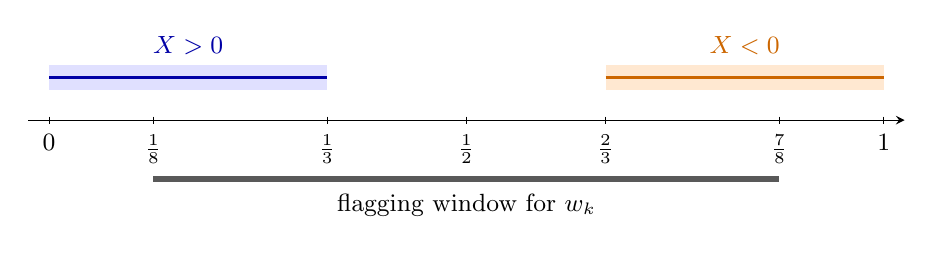
\begin{tikzpicture}[x=10.6cm,y=1cm,>=stealth,font=\small]
 \fill[blue!12] (0,.38) rectangle (0.333333,.7);
 \fill[orange!18] (0.666667,.38) rectangle (1,.7);
 \draw[blue!65!black,thick] (0,.54)--(0.333333,.54);
 \draw[orange!80!black,thick] (0.666667,.54)--(1,.54);
 \node[blue!65!black,above] at (.166667,.7) {$X>0$};
 \node[orange!80!black,above] at (.833333,.7) {$X<0$};
 \draw[->] (-.025,0)--(1.025,0);
 \foreach \x/\lab in {0/0,0.125/{\frac18},0.333333/{\frac13},0.5/{\frac12},0.666667/{\frac23},0.875/{\frac78},1/1}
  {\draw (\x,.045)--(\x,-.045);\node[below] at (\x,-.06) {$\lab$};}
 \draw[black!65,line width=2pt] (.125,-.75)--(.875,-.75);
 \node[below] at (.5,-.82) {flagging window for $w_k$};
\end{tikzpicture}
\caption{At the first flagged index, the true residue
$(2^kX/\Pi)\bmod1$ lies in the left interval for $X>0$ and the right
interval for $X<0$.  The circular error of $w_k$ is less than $2^{-10}$.
The flagging window excludes any approximation that wraps across $0=1$,
so the side of $1/2$ determines the sign.}
\label{fig:crt-sign}
\end{figure}

The first-flag condition uses one universal quantifier over smaller
short indices, raising the level for $w_k$ by one.  Existentially
quantifying a first flagged index with $w_k<1/2$, or with $w_k>1/2$,
raises it once more.  These tests return the positive or negative sign;
if neither succeeds, return zero.  This is the asserted
$\Flevel{\max(a,5)+3}$ procedure.
\end{proof}

\begin{corollary}[Signs of controlled integers]\label{cor:controlled-sign}
If a controlled family has no indeterminates, its sign is available,
uniformly in any short indices belonging to its input word.
\end{corollary}

\begin{proof}
Apply Proposition~\ref{prop:crt-sign} with the logarithmic norm bound
$b$ in place of $m$ and with the family's cutoff $\lambda$.
\end{proof}

We can now manipulate polynomials through short bounds and modular
evaluation procedures.  The next step is to show that a characteristic
polynomial of multiplication in a finite polynomial quotient admits
exactly this description, even when the quotient has exponentially
large rank.
